\section{The Algorithm}
\label{sec:algorithm}

In this section, we will briefly describe the steps our algorithm takes and then provide more details on key parts of it. The algorithm consists of two parts, a \emph{Compress} function and a \emph{Decompress} function. In the Compress function, to which one passes the original image as an argument, the following steps are completed:
\begin{enumerate}
\item \emph{Feature extraction}. First, we add rows and columns to the image matrix so that the number of rows and columns is evenly divisible by the predefined patch size. We then extract patches of size {\color{red}X by X} and return them as a single column vector.

\item \emph{Training} is performed ``globally'', with much more images as input than just the one we want to compress. However, as it is always possible to add several training epochs on the current image in addition to the already trained matrix, we list training in this spot. The training function chooses several columns of our patches matrix and uses them as input for the neural network while the target output is the same column vector. The weights are set accordingly during the training phase until the difference between the output and the target vector is within a desired threshold.

\item \emph{Network separation}. After the training is done, we separate the neural network into two parts, one including input and hidden layer and the other including hidden and output layer. The first will be our compression network, using the values of the hidden layer as the output, while the latter is the decompression network, taking the values of the hidden layer as input and returning an approximation of the original data.

\item \emph{Compression} is done by applying the compression network to the column vectors of the image.

\item \emph{Quantization}. After compression, we are presented with values in the range of \([-1, 1]\). 
\end{enumerate}


Different learning methods were tried like {\color{red}TODO} but it turned out that for the Levenberg-Marquardt method the results were best. 


%%\subsection{Singular Value Decomposition}
%%The singular value decomposition(SVD) is a matrix factorization. A m$\times$n matrix M can be written as a product of three matrices U, $\Sigma$ and V$^*$, where U is a unitary m$\times$m matrix, V$^*$ is the conjugate transpose of a n$\times$n unitary matrix V and $\Sigma$ is a m$\times$n diagonal matrix. The entries on the diagonal of $\Sigma$, which are non-negativ real numbers, are called the singular values of M. The columns of U are called left singular vectors and the rows of V$^*$ are called right singular vectors of M. \\
%%SVD can be used for image compression the following way. The singular values are sorted in descending order and then only the largest singular values and the corresponding right and left singular vectors are used to save the image.

\subsection{Quanitization}
\label{sec:quanitization}
\begin{figure}[tbp]
  \centering
  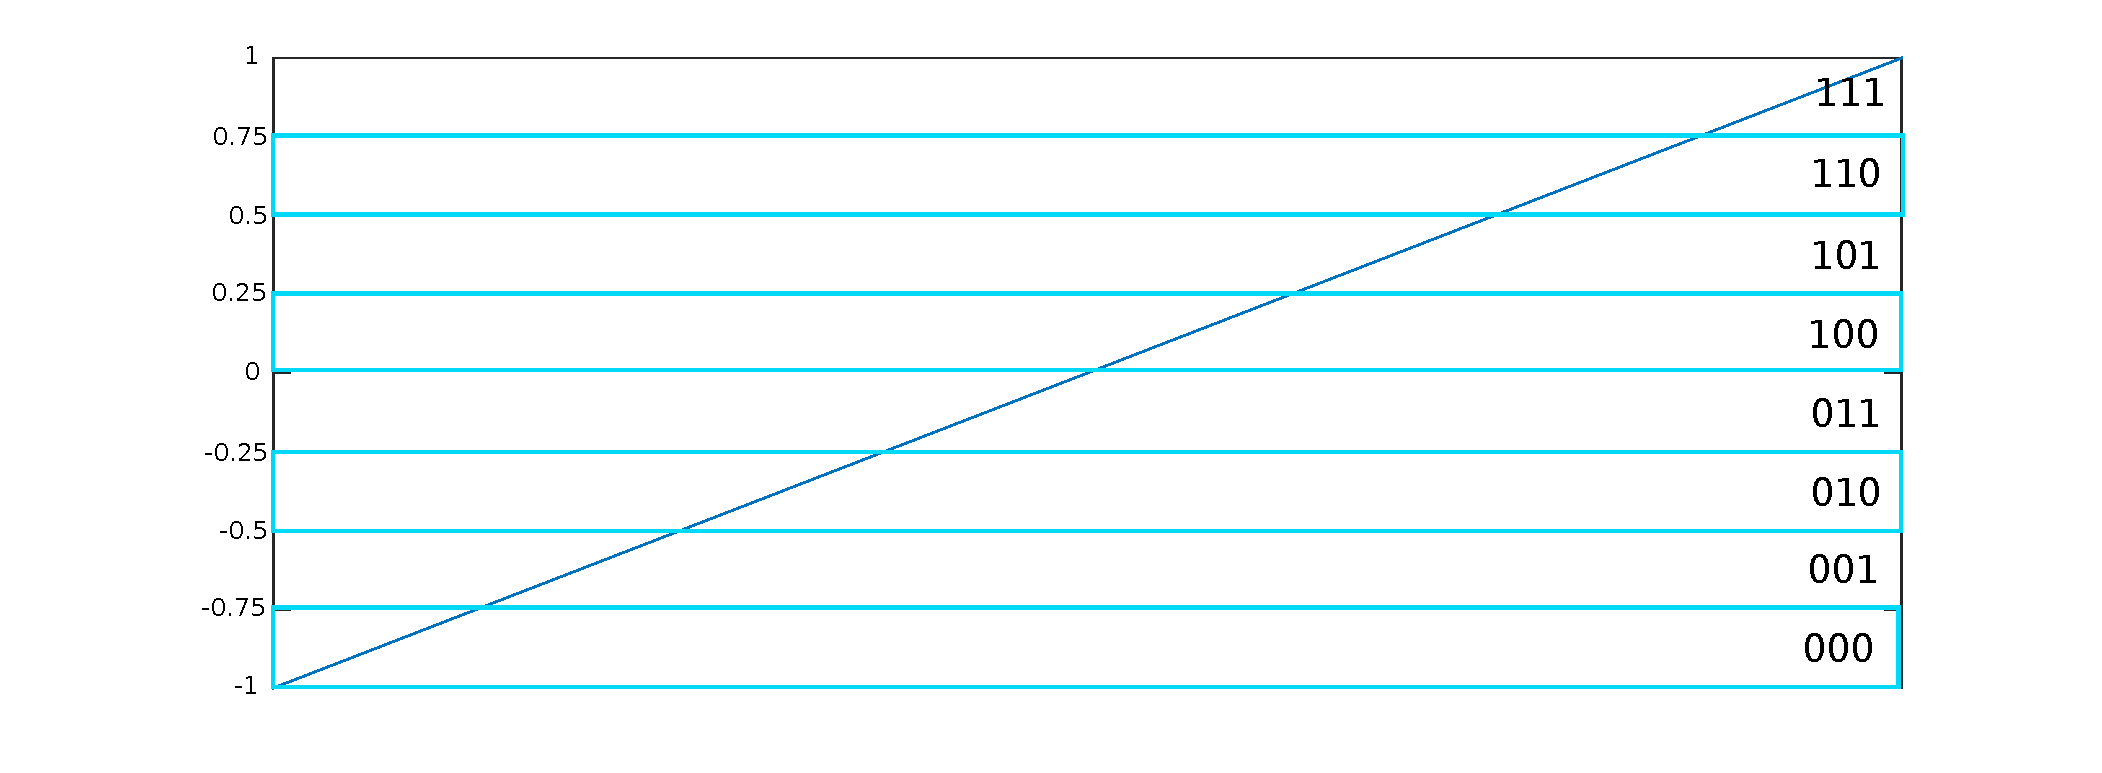
\includegraphics[width=\columnwidth]{images/bqQuantizer}
  \caption{Neural Network Structure for compression.}
  \label{fig:bpQuantizer}
\end{figure}

Quantization as shown in Figure~\ref{fig:bpQuantizer} is the process of mapping a large set of values to a smaller set of values. With this operation, we loose some precision but can reduce data size significantly. We construct 16 possible binary codes which can be represented with 4 bits. Each code represents a subinterval between the real values -1 and 1. This way, we use 4 bits for a pixel that originally is represented by 8 bits.  

\subsection{Compression with neural networks}
We use the topology described in section~\ref{sec:neural_net_structure}. This network is then trained with a set of random images. Then, the image can be compressed with this network in the following way. Chunks of the image are iterated in turn and every chunk is fed into the neural network from the left hand side. If we have 8$\times$8 chunks, we have 64 pixels and each pixel is given to one node on the input layer(which in this case has 64 nodes) of the neural network. Then the values on the hidden layer are taken as the "compressed" values. Since the hidden layer has fewer nodes than the input layer, this gives a compression. As one can see in Figure ~\ref{fig:nnStructure}, the neural net used here has 16 nodes on the hidden layer. This already gives a compression ratio of 0.25. 

TODO: Describe that one needs to separate neural network for compression and decompression?

\subsection{Compression with quantization}
To further improve compression, quantization as described in Section~\ref{sec:quanitization} is used. The output of the neural network is quantized, such that each 8 bit value is represented using 3 bits.  

\subsection{The Compression Algorithm}
\label{sec:compAlg}

Overall, the compression can be summarized as follows.

\begin{enumerate}
\item The neural network is trained with the training set; in this case 100 images.
\item The trained network is adjusted to the actual image by selecting a few random chunks of the image. Then, the the training is done with those few chunks and the weights updated. 
\item Compress 8$\times$8 chunks of image in turn using neural network.
\item Compress all the resulting values with quanitization.

\end{enumerate}

\subsection{Decompression}
\label{sec:decompAlg}
TODO: Describe how the decompression works
